\subsection{ Przykłady przekształceń geometrycznych w dwuwymiarowej przestrzeni euklidesowej}

Do elementarnych przekształceń w dwuwymiarowej przestrzeni euklidesowej ($\mathbb{R}^{2}$) możemy zaliczyć \textit{translację} (przesunięcie), zmianę skali obiektu, bądź jego rotację \citep[s. 2]{Glowacki2013}.

W przypadku translacji danemu punktowi A w $\mathbb{R}^{2}$ postaci: $A(x_{1}, y_{2})$ przyporządkowuje się nową pozycję poprzez dodanie do współrzędnych punktu A wielkość przesunięcia ($d_{x}$). W wyniku tego otrzymujemy nowy punkt A' postaci: A'($x'_{1}, y'_{2}$). Przedstawiono to na rysunku poniżej.


\begin{figure}[H]
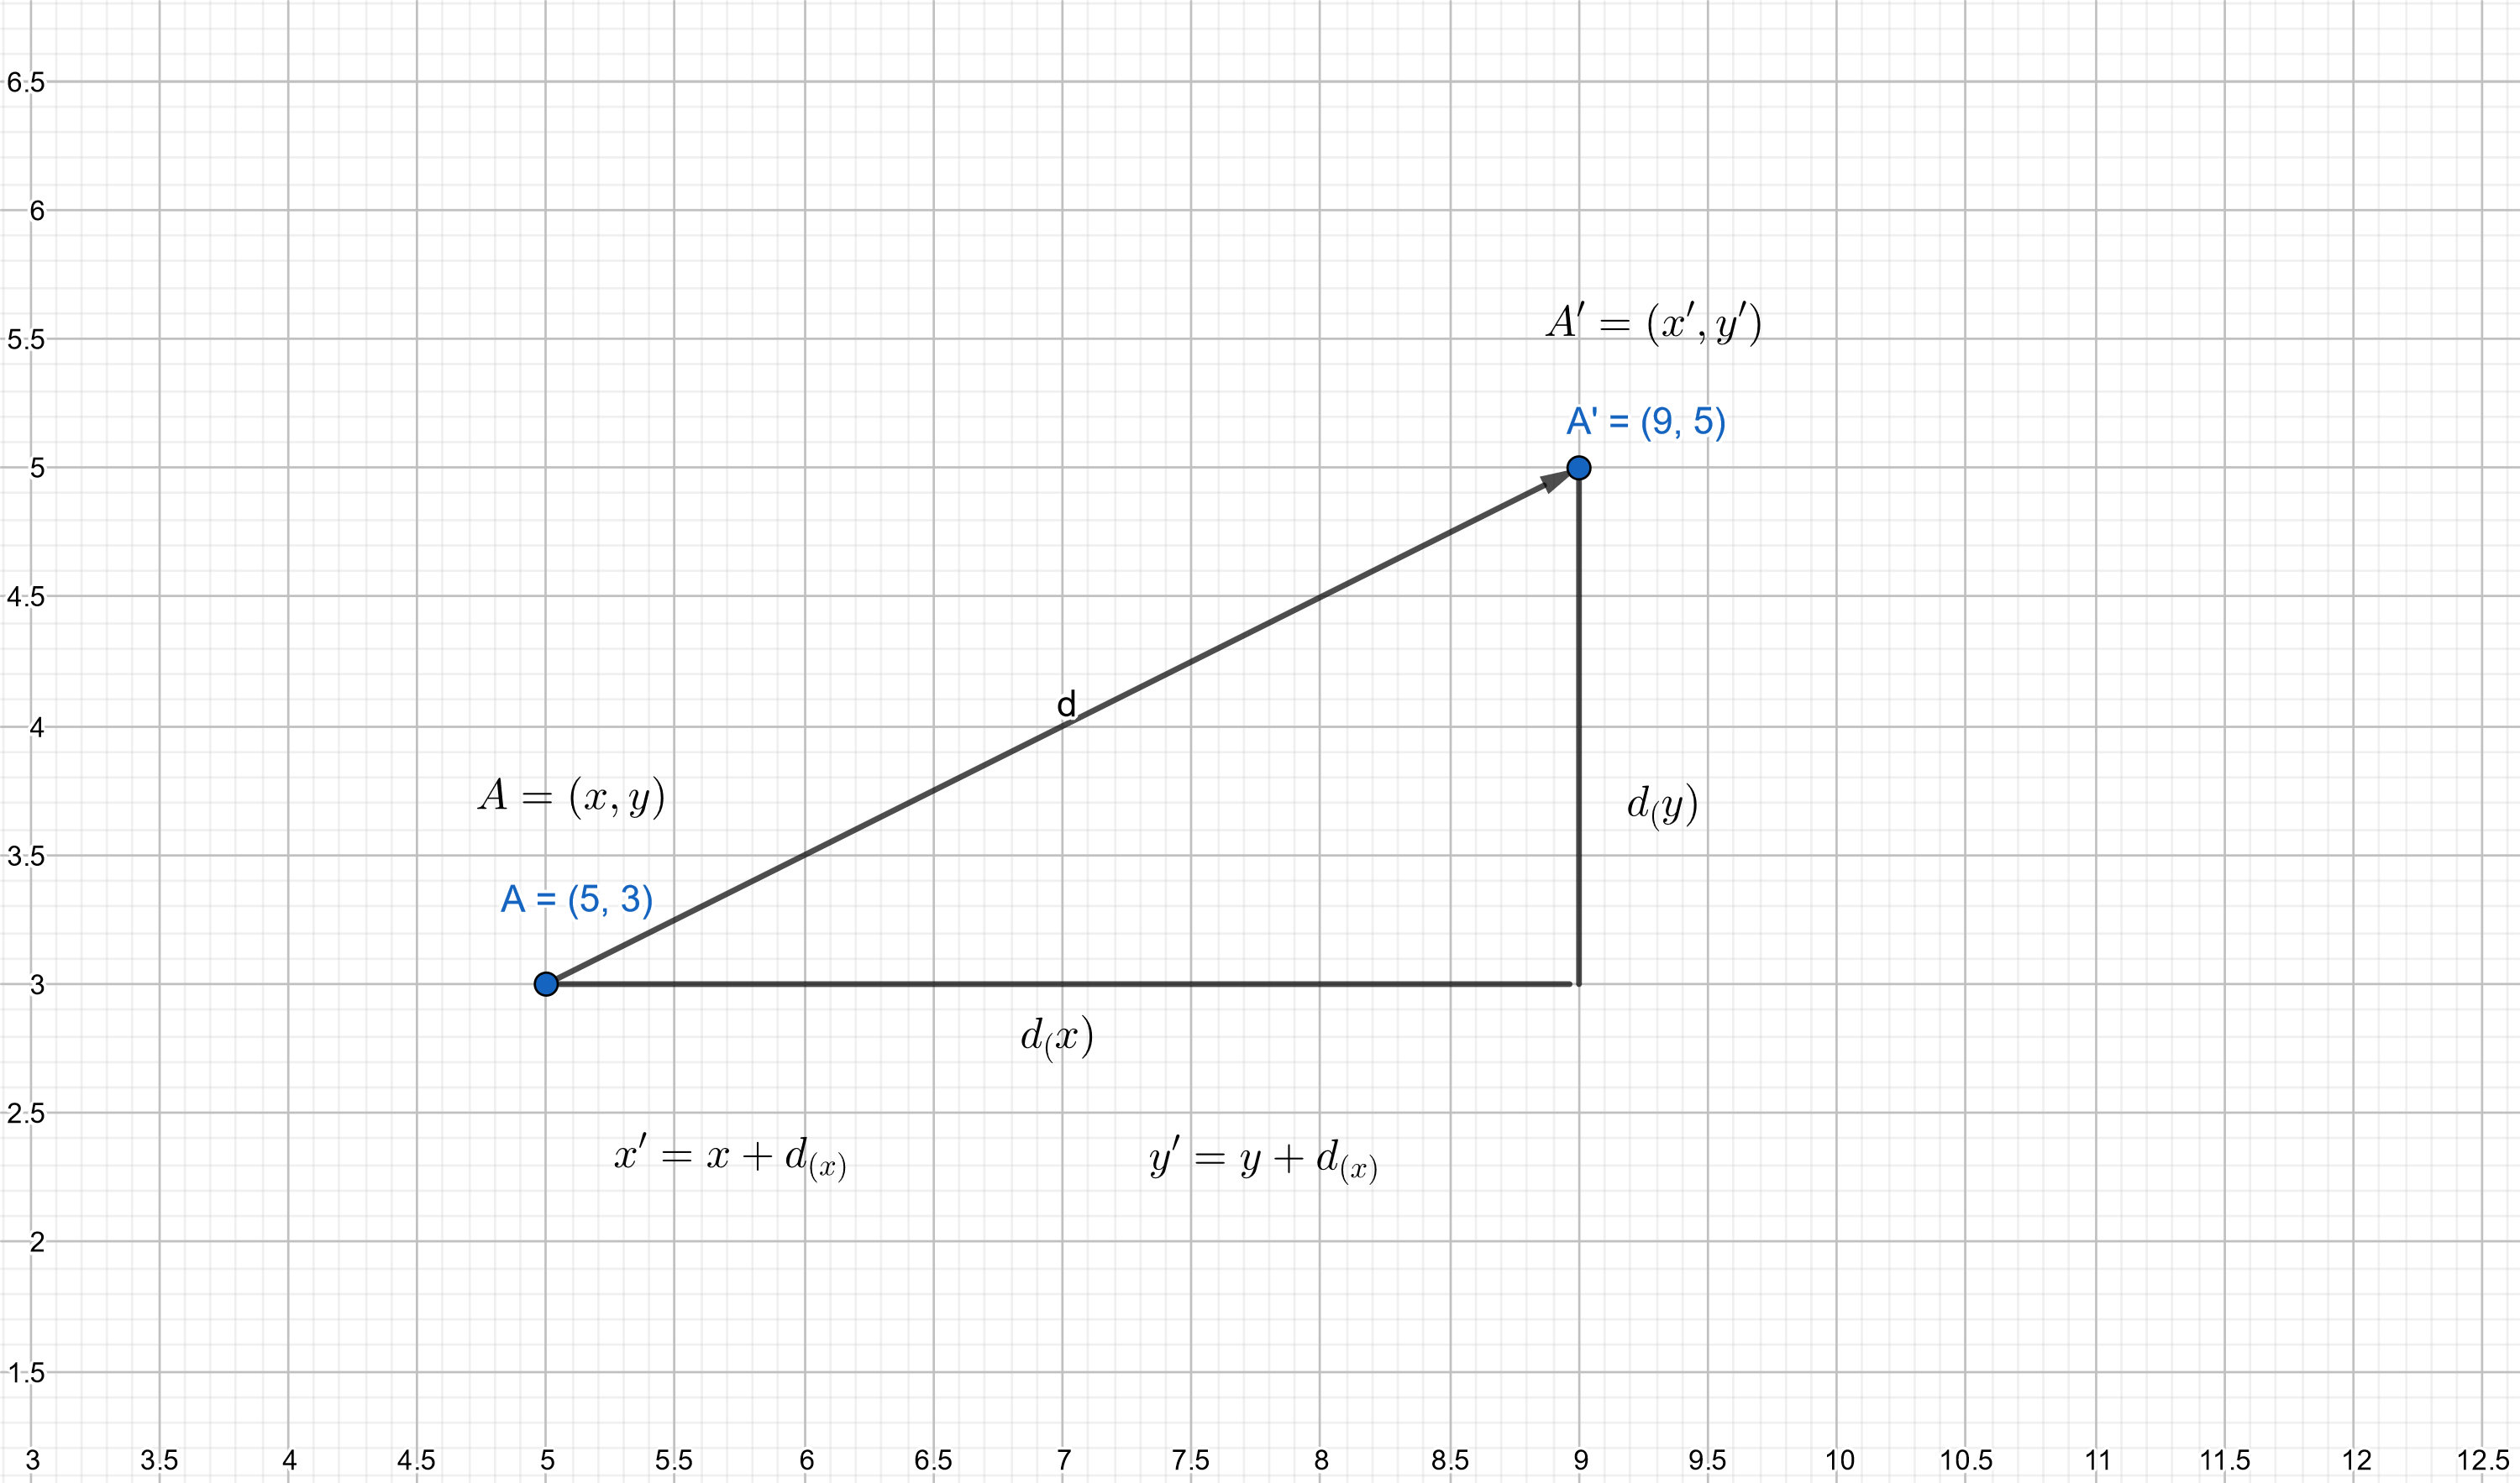
\includegraphics[width=\textwidth]{przesuniecie.png}
\caption{Przesunięcie punktu $A(5,3)$ do $A'(9,5)$ w dwuwymiarowej przestrzeni euklidesowej $\mathbb{R}^{2}$. Rysunek wykonano za pomocą programu GeoGebra. Źródło: Opracowanie własne na podstawie \citep[s. 4]{Badura2005} i \citep[s. 3]{Glowacki2013}}
\centering
\end{figure}

Skalowanie jest operacją modyfikującą proporcję obrazu względem początku układu współrzędnych. Polega na przesunięciu obiektu względem dowolnie wybranego stałego punktu. Jest nim zwykle początek układu współrzędnych, czyli punkt $(0,0)$. Ten rodzaj skalowania nazywamy \textit{skalowaniem względem początku układu współrzędnych}.

Obiekty geometryczne można skalować przy za pomocą współczynników $s_{x} \neq 0$ w kierunku osi $OX$ i $s_{y} \neq 0$ w kierunku osi $OY$. Skalowanie względem początku układu współrzędnych to inaczej transformacja odwzorowująca dowolnie wybrany punkt $P(x,y)$ na punkt $P'(x',y')$ przez pomnożenie współrzędnych $x$ i $y$ punktu $P$ przez stałe, niezerowe współczynniki skalowania $s_{x}$ i $s_{y}$.

Współczynnik skalowania s może zwiększać odległość obiektu względem punktu $(0,0)$ jeśli zachodzi nierówność $|s| > 1$ lub zmniejszać tę odległość jeśli $|s| < 1$. Natomiast jeśli $s_{x} = s_{y}$ to skalowanie nazywamy \textit{jednorodnym}. W przeciwnym wypadku, czyli $s_{x} \neq s_{y}$ skalowanie nazywamy niejednorodnym.

Jeśli zdecydujemy się przedstawić współrzędne punktów $P$ i $P'$ jako wektory kolumnowe to skalowanie może się odbyć jako mnożenie macierzy przez macierz. Współrzędne punktu $P$ możemy wtedy zapisać wzorami jako:

\begin{equation*}
    \begin{bmatrix}
    x' \\
    y'
    \end{bmatrix}
    =
    \begin{bmatrix}
    s_{x} & 0 \\
    0 & s_{y}
    \end{bmatrix}
    \cdot
    \begin{bmatrix}
    x \\
    y
    \end{bmatrix}
\end{equation*}

Macierz:
\begin{equation*}
S(s_{x}, s_{y}) =
    \begin{bmatrix}
    s_{x} & 0 \\
    0 & s_{y}
    \end{bmatrix}
\end{equation*}

nazywamy \textit{macierzą skalowania}. Uogólniając powyższe operacje możemy zapisać, że:
\begin{equation*}
    P' = S(s_{x}, s_{y}) \cdot P
\end{equation*}
\citep[s. 4-5]{Badura2005}.

Przykład przedstawiono na rysunku poniżej.

\begin{figure}[H]
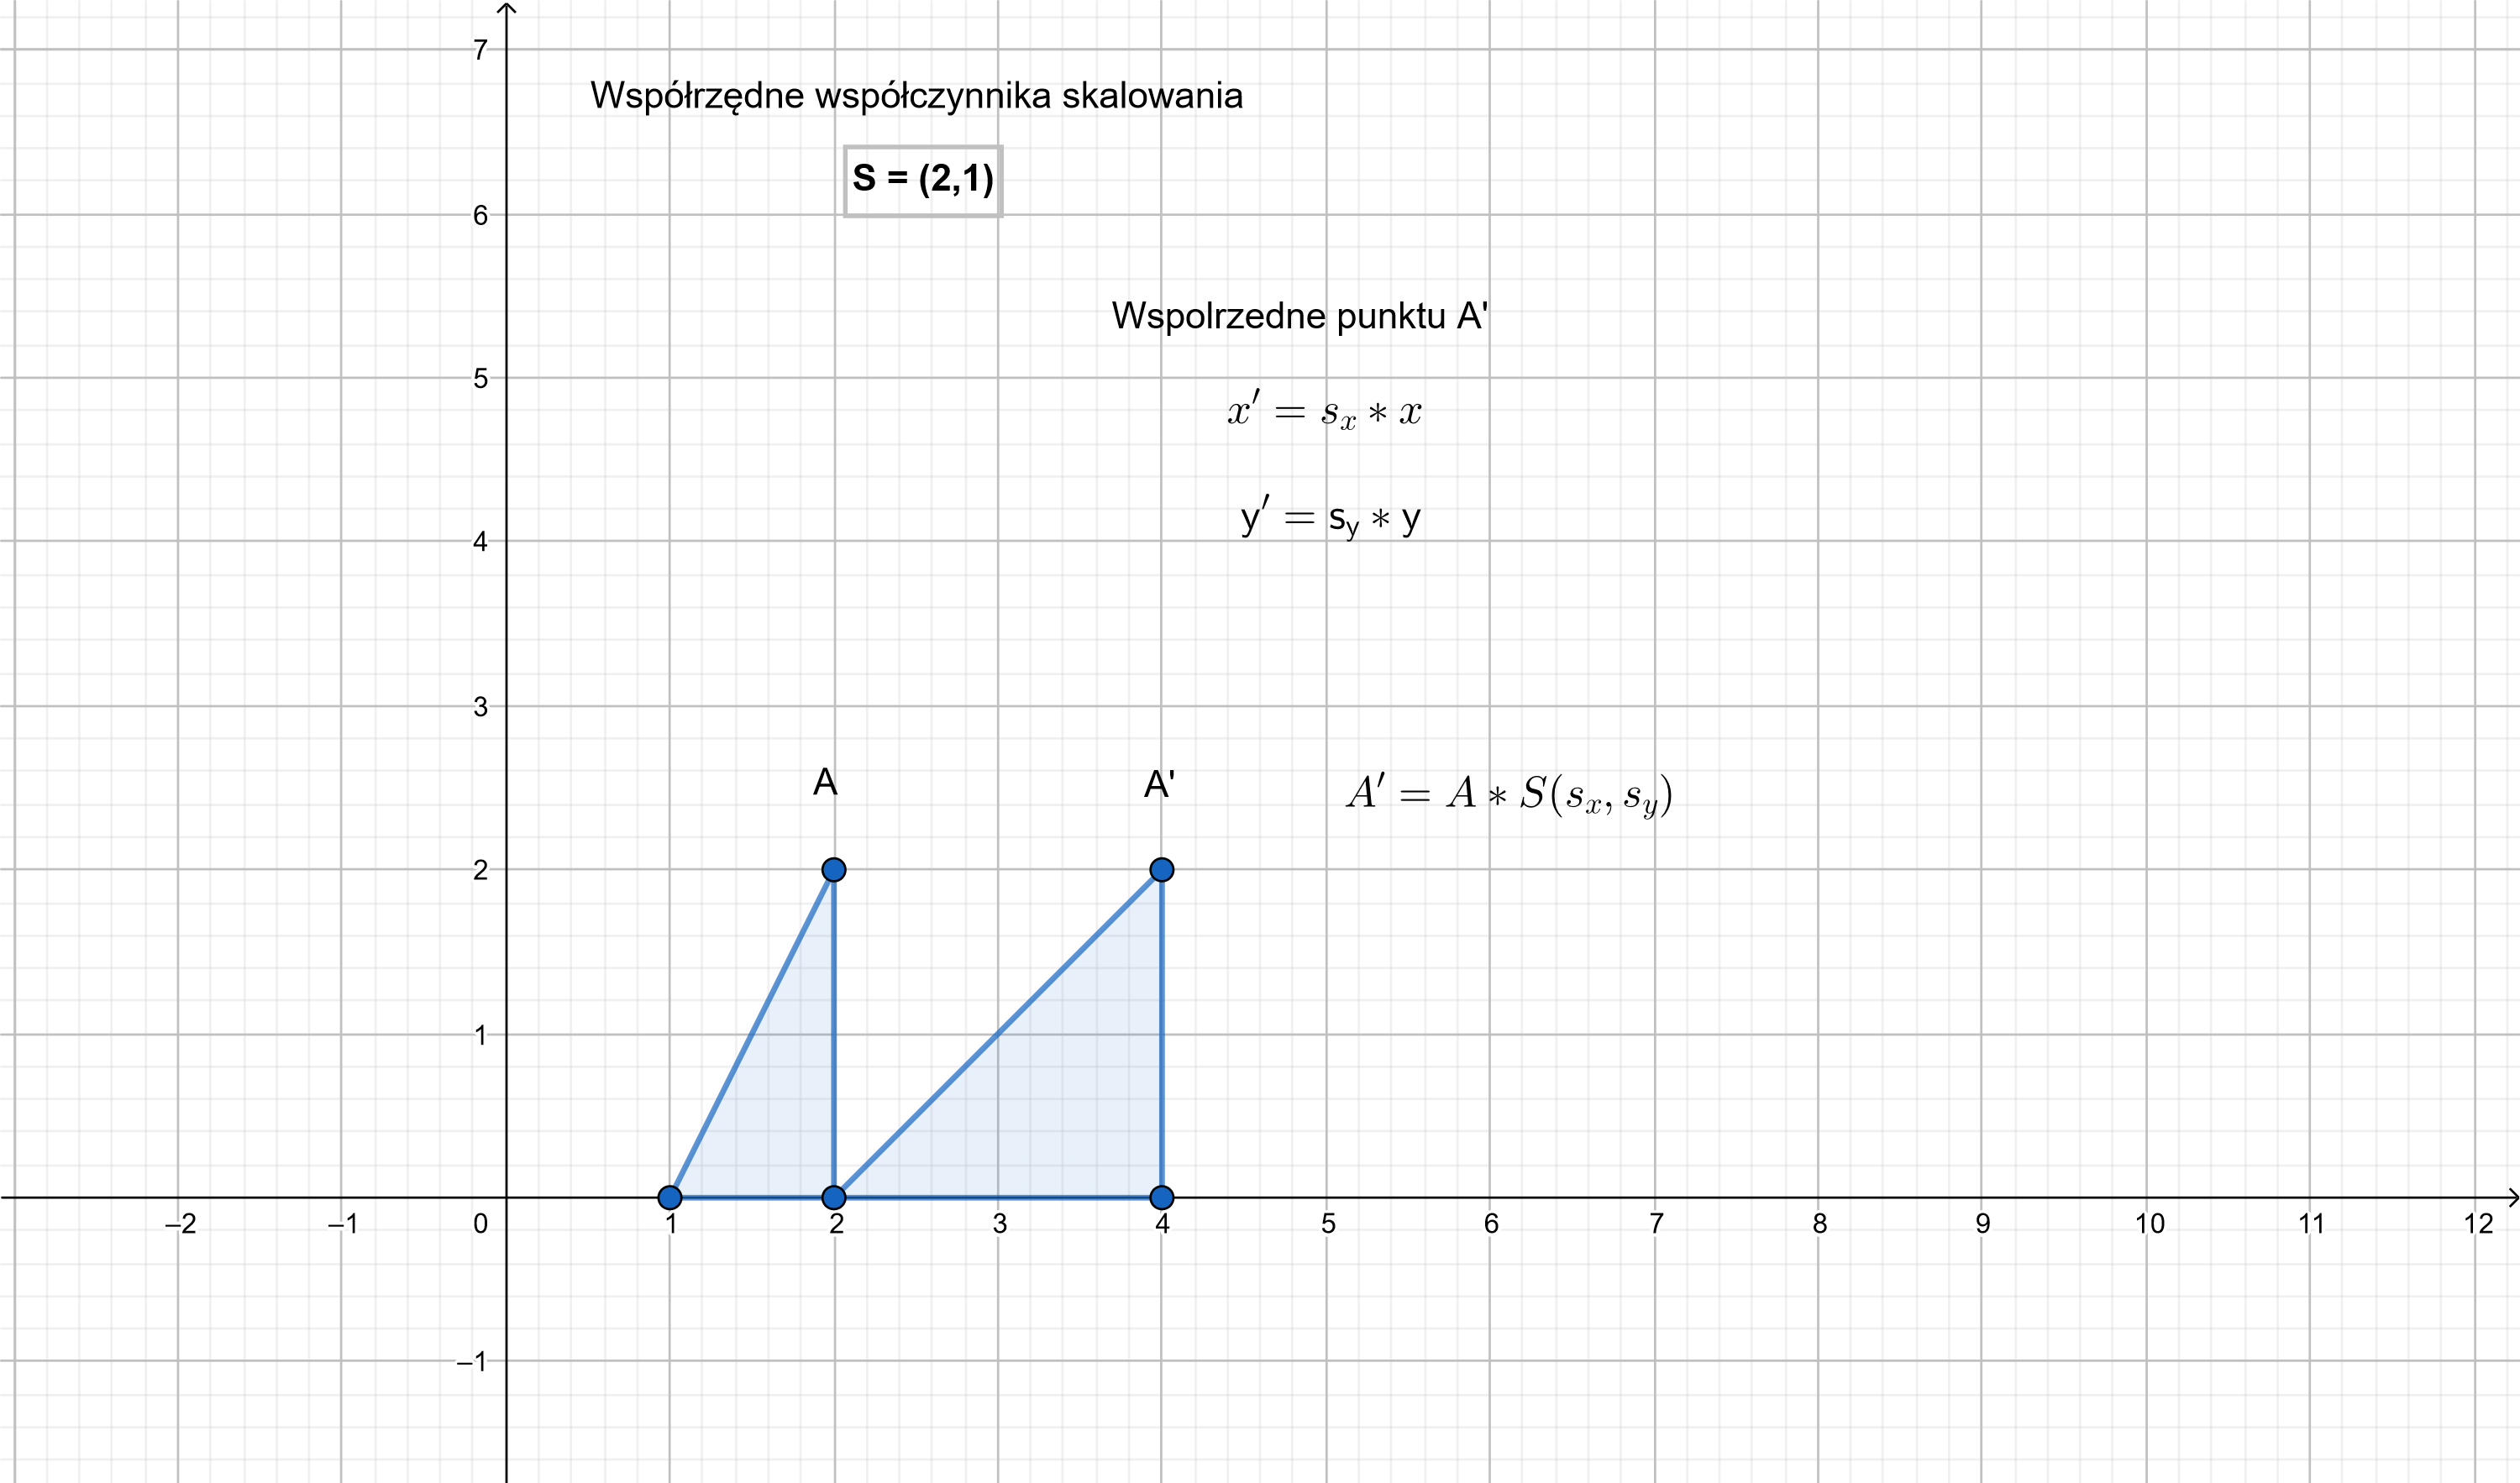
\includegraphics[width=\textwidth]{skalowanie.png}
\caption{Skalowanie trójkąta A do trójkąta A' względem początku układu współrzędnych i S(2,1). Rysunek wykonano za pomocą programu GeoGebra. Źródło: Opracowanie własne na podstawie \citep[s. 4-5]{Badura2005}} 
\centering
\end{figure}

Ostatnią z operacji jaką chciałbym opisać są obroty figur w $\mathbb{R}^{2}$. Wyróżniamy obroty względem początku układu współrzędnych lub wokół punktu.

Obrót względem początku układu współrzędnych to operacja polegająca na obrocie poszczególnych punktów obiektu o odgórnie ustalony kąt $\phi$.

Formalnie obrotem wokół początku układu współrzędnych nazywamy przekształcenie odwzorowujące punkt $P(x,y)$ na punkt $P'(x',y')$ w taki sposób, że odległości punktów $P$ i $P$' od początku układu współrzędnych $O$ spełniają równość $\overline{|OP|} = \overline{|OP'|}$, a kąt między odcinkami $\overline{OP}$ i  $\overline{OP'}$ jest równy wartości kąta $\phi$. Ponieważ istnieją dwa możliwe obrazy punktu $P$ spełniające powyższe warunki przyjęło się, że obrót o kąt dodatni wykonuje się w kierunku przeciwnym do ruchu wskazówek zegara \citep[s. 5 - 6]{Badura2005}.

Współrzędne Punktu P dane są wzorami:
\begin{equation}
    x' = x\cos\phi - y\sin\phi, \quad y' = x\sin\phi + y\cos\phi
\end{equation}

Obrót wokół początku układu współrzędnych o kat $\phi$ można wyrazić za pomocą macierzy
\begin{equation*}
    \begin{bmatrix}
    x' \\
    y'
    \end{bmatrix}
    = 
    \begin{bmatrix}
    \cos\phi & -\sin\phi \\
    \sin\phi & \cos\phi
    \end{bmatrix}
    \cdot
    \begin{bmatrix}
    x \\
    y
    \end{bmatrix}
\end{equation*}
\\
Poniższa macierz:
\begin{equation*}
    R(\phi) = 
    \begin{bmatrix}
    \cos\phi &  -\sin\phi \\
    \sin\phi & \cos\phi
    \end{bmatrix}
\end{equation*}

Jest \textit{macierzą obrotu}. Opisuje ona  obrót danego wektora (punktu) w przestrzeni $\mathbb{R}^{2}$.
Zadanie obrotu Punktu P wokół początku układu współrzędnych możemy krótko zapisać jako:
\begin{equation*}
    P' = R(\phi) \cdot P
\end{equation*}

Obrót wokół początku układu współrzędnych o kąt $\phi$ i odpowiadającą temu obrotowi macierz R będziemy oznaczać poprzez zapis $R(\phi)$ \citep[s. 6-7]{Badura2005}.

Przykład przedstawiono na poniższym rysunku.

\begin{figure}[H]
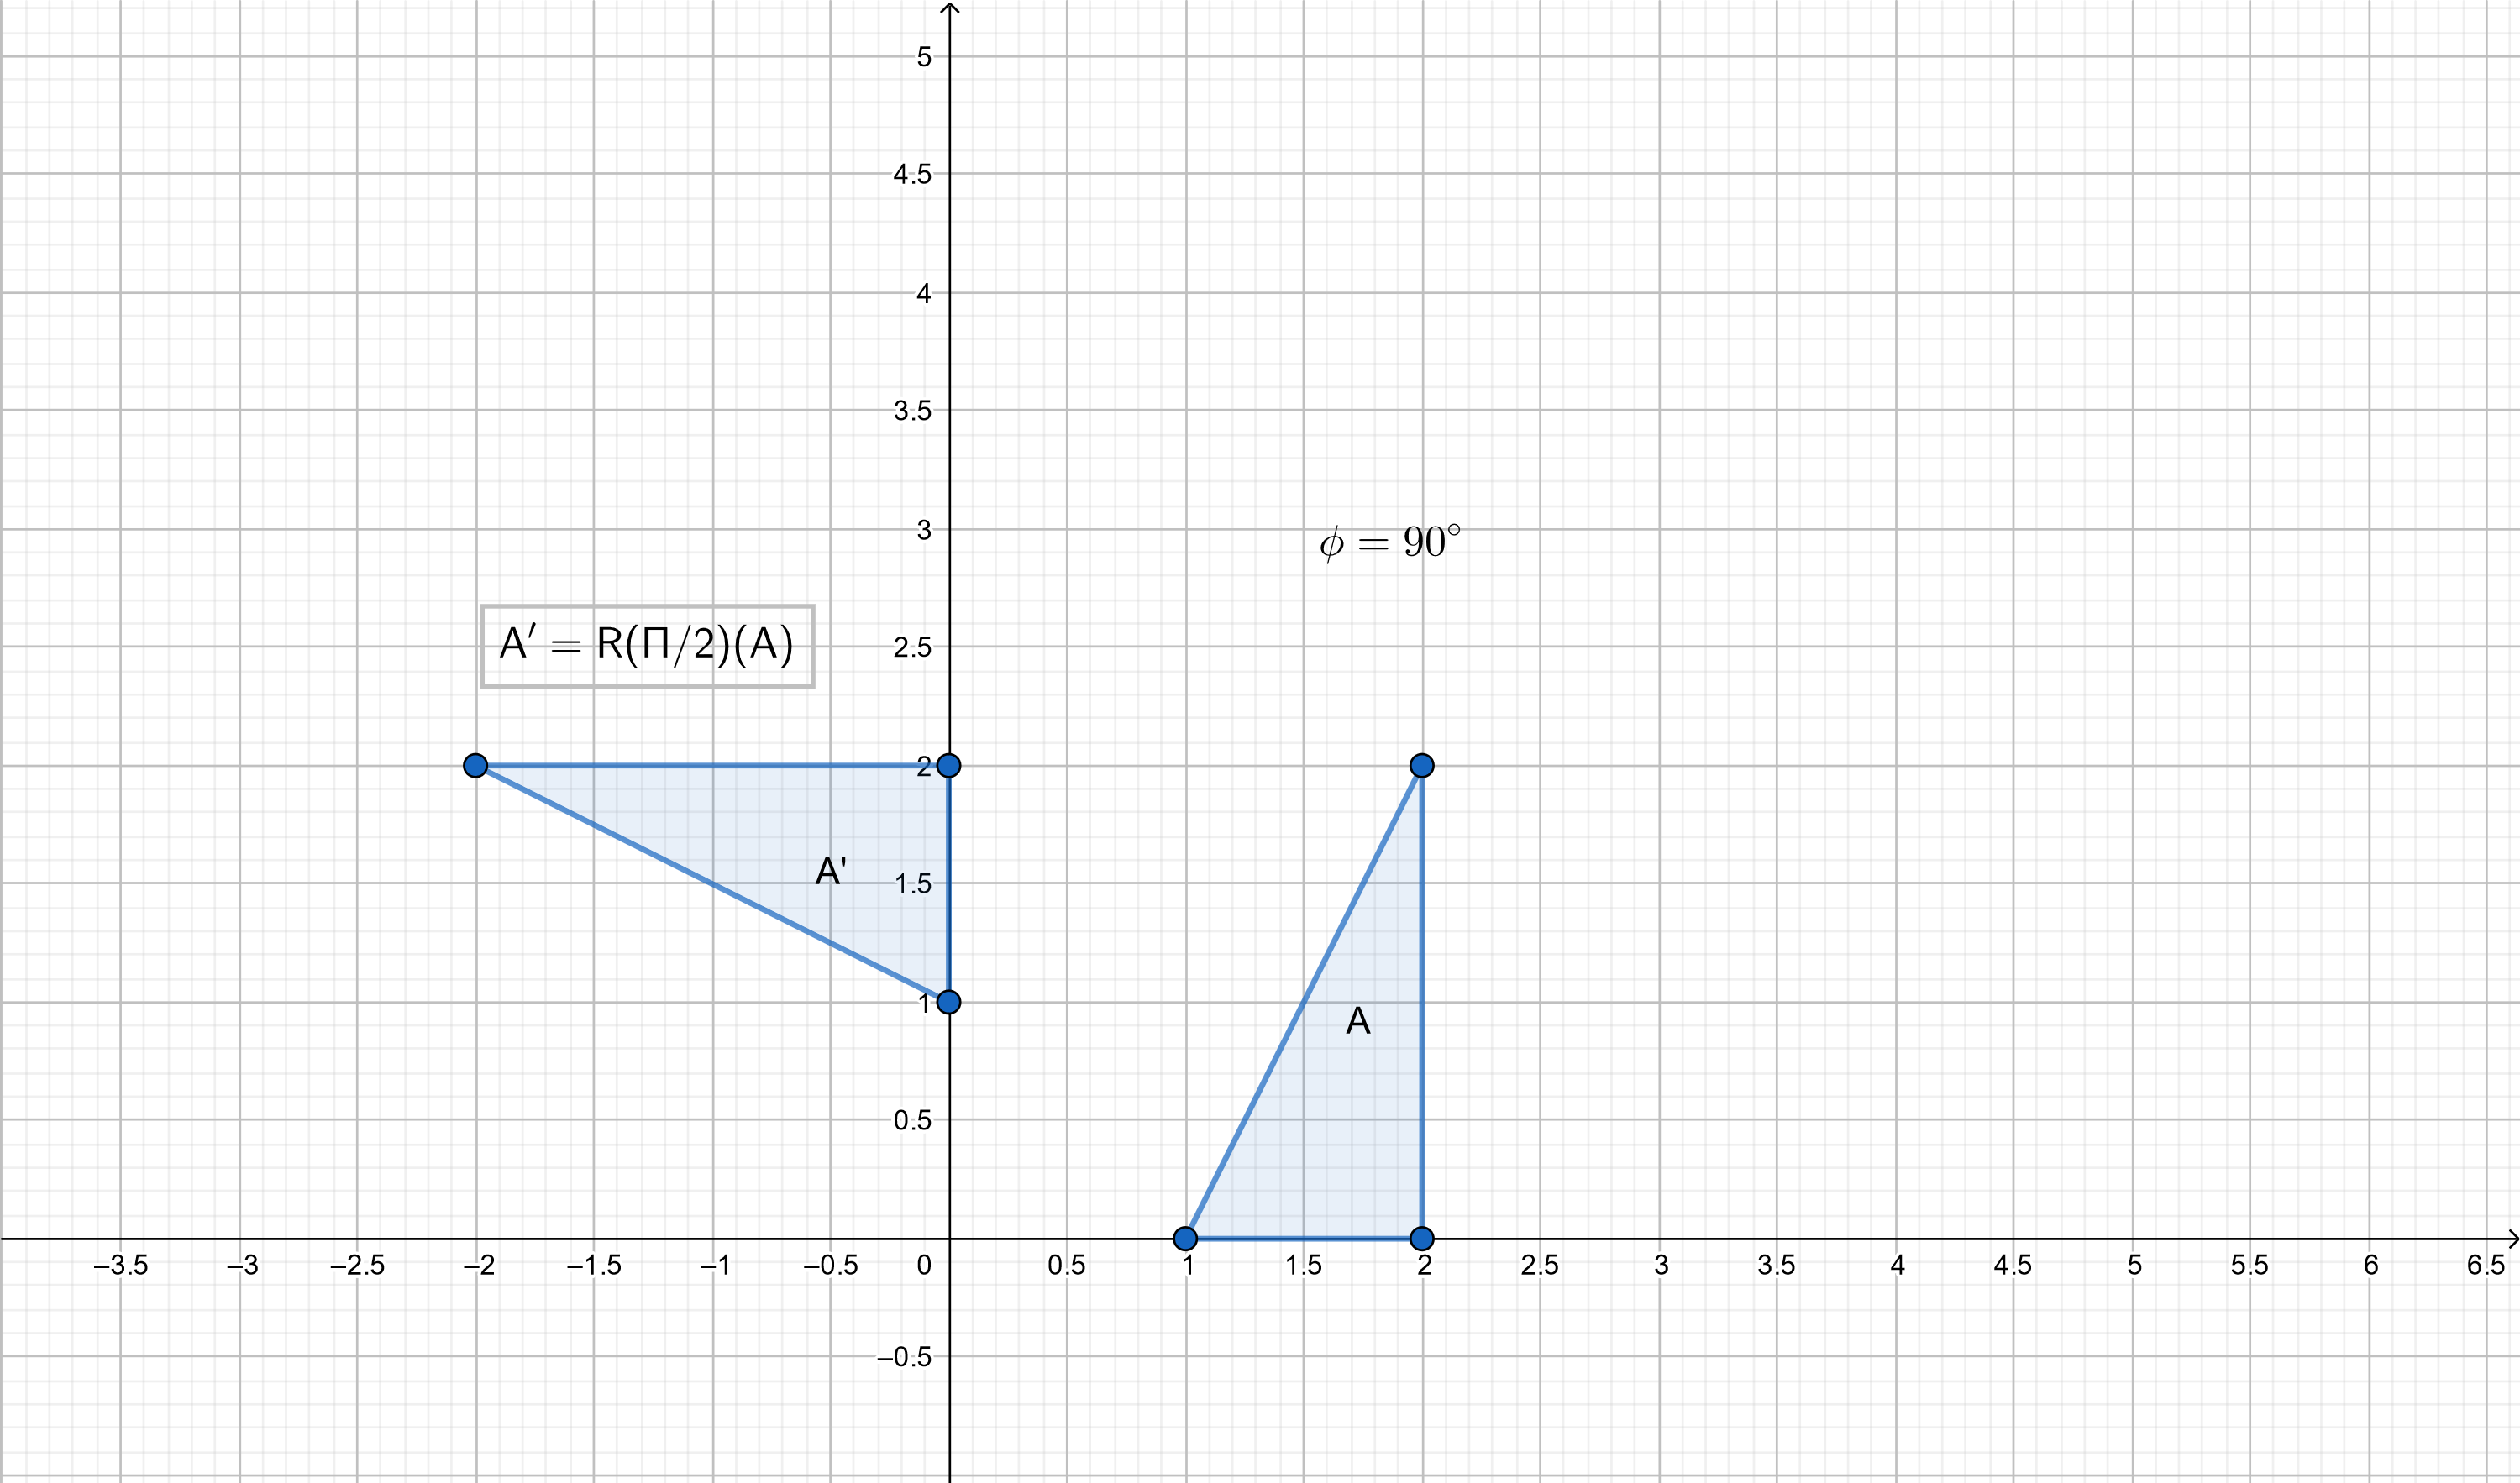
\includegraphics[width=\textwidth]{obrot.png}
\caption{Obrót trójkąta $A$ do trójkąta $A'$ względem początku układu współrzędnych o kąt $90^{\circ}$. Rysunek wykonano za pomocą programu GeoGebra. Źródło: Opracowanie własne na podstawie \citep[s. 6-7]{Badura2005}} 
\centering
\end{figure}


\subsubsection{Obrót wokół dowolnego punktu}

Mając do dyspozycji Punkt P o współrzędnych ($x_{0}$ i $y_{0}$)  i jakiś dowolny obiekt możemy spróbować obrócić go wokół punktu $P$ o kąt $\phi$.
Aby to wykonać potrzebujemy wykonać sekwencyjnie trzy przekształcenia:

\begin{enumerate}
    \item Przesunąć punkt $P$ na początek układu współrzędnych,
    \item Obrót wokół początku układu współrzędnych o podany kąt $\phi$,
    \item Ponowne przesunięcie płaszczyzny w taki sposób żeby Punkt $P$ powrócił do swojego położenia wyjściowego.
\end{enumerate}

Zatem wykonujemy najpierw przesunięcie o wektor $[-x_{0}, -y_{0}]$ aby następnie wykonać obrót wokół początku układu współrzędnych. Na koniec przesuwamy ponownie punkt P o $[x_{0}, y_{0}]$.
Zapisując te działania bardziej formalnie dochodzimy do następujących wzorów\footnote{\citep[s. 9 - 10]{Badura2005}.}:

\begin{equation*}
    x' = (x - x_{0})\cos\phi - (y - y_{0})\sin\phi + x_{0}
\end{equation*}
\begin{equation*}
    y' = (x - x_{0}\sin\phi + (y - y_{0})\cos\phi + y_{0}
\end{equation*}

Obrót wokół dowolnego punktu o współrzędnych ($x_{0}$, $y_{0}$) o kąt $\phi$ będziemy oznaczać przez zapis $R_(x_{0},y_{0})$($\phi$) \citep[s. 10]{Badura2005}.
\\
Graficzne rozwiązanie problemu przedstawia poniższy rysunek:

\begin{figure}[H]
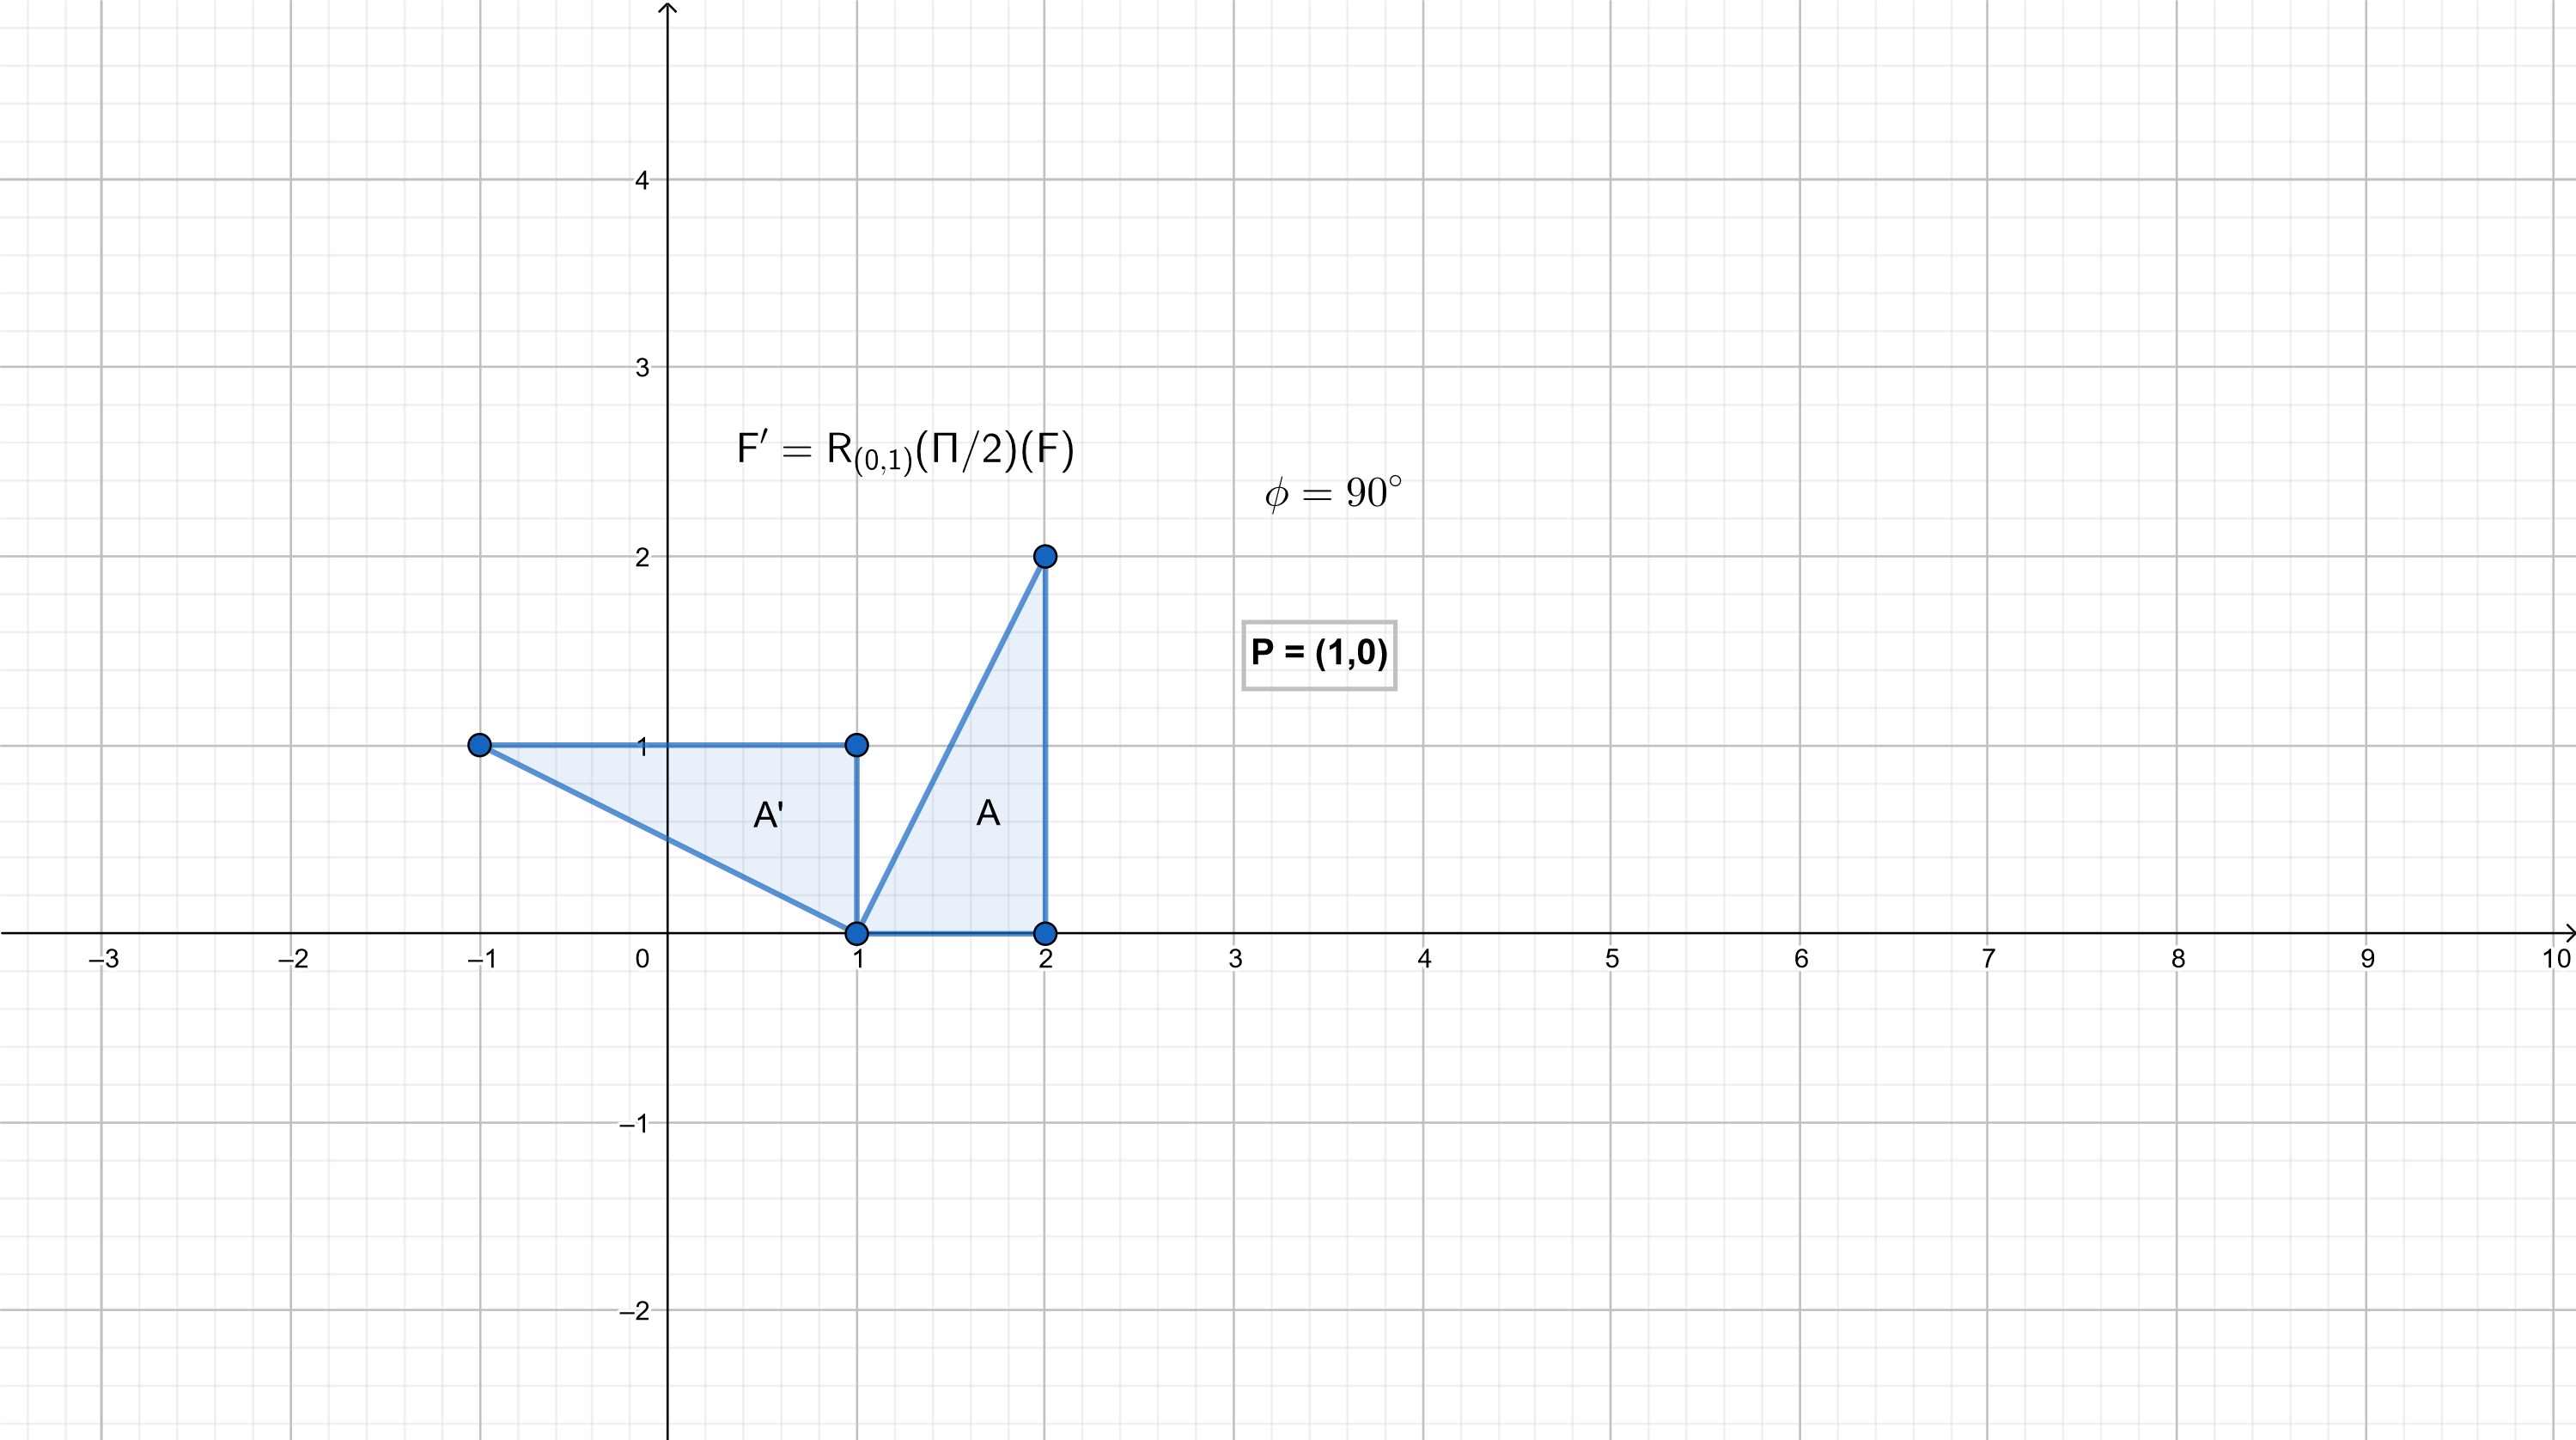
\includegraphics[width=\textwidth]{obrot2.png}
\caption{Obrót trójkąta $A$ do trójkąta $A'$ względem punktu $P (1,0)$ o kąt $90^{\circ}$. Rysunek wykonano za pomocą programu GeoGebra. Źródło: Opracowanie własne na podstawie \citep[s. 9-10]{Badura2005}} 
\centering
\end{figure}